\section{Development Pipeline}

This section outlines the overall design pipeline adopted for developing the integrated ESP32 TTGO T-Display device with a custom 3D-printed housing. The pipeline consists of four sequential phases: system analysis, mechanical design, electrical integration, and programming. Each phase builds directly on the outputs of the preceding one, ensuring coherent integration across hardware, mechanical, and software domains. The complete pipeline is summarised in Figure~\ref{fig:development_pipeline}.

\begin{figure}[H]
    \centering
    \begin{tikzpicture}
    [
        node distance=0.6cm,
        box/.style={
            draw, rectangle, rounded corners=4pt,
            minimum width=5.5cm, minimum height=1.0cm,
            text centered, font=\small\bfseries,
            fill=gray!15, line width=0.8pt
        },
        subbox/.style={
            draw, rectangle, rounded corners=3pt,
            minimum width=4.8cm, minimum height=0.75cm,
            text centered, font=\small,
            fill=white, line width=0.5pt
        },
        arrow/.style={->, >=stealth, line width=1pt},
        phase/.style={font=\footnotesize\itshape, text=gray}
    ]

    % Phase 1 – System Analysis
    \node[box] (sa) {Phase 1: System Analysis};
    \node[subbox, below=0.2cm of sa] (sa1) {Board dimension inspection};
    \node[subbox, below=0.2cm of sa1] (sa2) {Architectural specification review};

    % Phase 2 – Mechanical Design
    \node[box, below=0.6cm of sa2] (md) {Phase 2: Mechanical Design};
    \node[subbox, below=0.2cm of md] (md1) {CAD modelling (Fusion 360)};
    \node[subbox, below=0.2cm of md1] (md2) {Slicing and print-parameter setup (Cura)};
    \node[subbox, below=0.2cm of md2] (md3) {FDM printing (Ender 3 V2, PLA)};

    % Phase 3 – Electrical Integration
    \node[box, below=0.6cm of md3] (ei) {Phase 3: Electrical Integration};
    \node[subbox, below=0.2cm of ei] (ei1) {Component wiring};

    % Phase 4 – Programming
    \node[box, below=0.6cm of ei1] (pg) {Phase 4: Programming};
    \node[subbox, below=0.2cm of pg] (pg1) {User interface design and implementation (Arduino IDE)};
    \node[subbox, below=0.2cm of pg1] (pg2) {Application development and integration};

    % Arrows between phases
    \draw (sa)  -- (sa1);
    \draw (sa1) -- (sa2);
    \draw[arrow] (sa2) -- (md);
    \draw (md)  -- (md1);
    \draw (md1) -- (md2);
    \draw (md2) -- (md3);
    \draw[arrow] (md3) -- (ei);
    \draw (ei)  -- (ei1);
    \draw[arrow] (ei1) -- (pg);
    \draw (pg)  -- (pg1);
    \draw (pg1) -- (pg2);

    \end{tikzpicture}
    \caption{Development pipeline for the integrated ESP32 TTGO T-Display device.}
    \label{fig:development_pipeline}
\end{figure}

\subsection{System Analysis}

The development process begins with a thorough analysis of the TTGO T-Display ESP32 board, which serves as the core component of the system. This phase involves a detailed inspection of the board's physical dimensions, including its overall footprint, the positions of connectors, buttons, and the integrated display, as well as any protrusions that must be accommodated by the enclosure.

\begin{figure}[H]
    \centering
    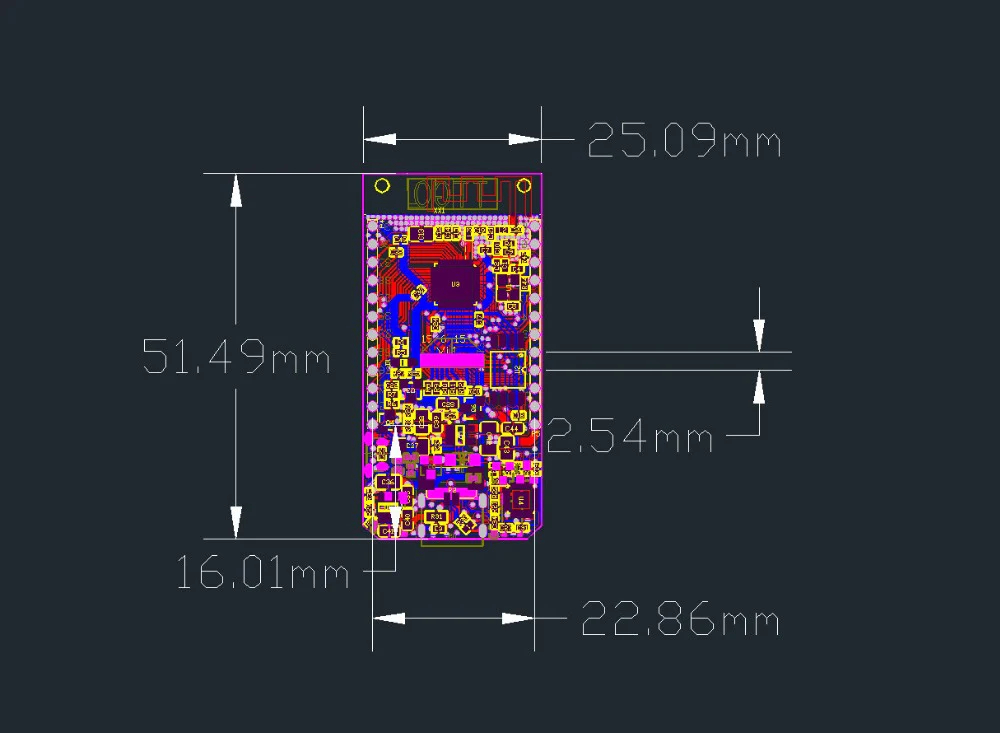
\includegraphics[width=0.5\textwidth]{development-testing/development/image/esp32ttgo_dimension.png}
    \caption{TTGO T-Display ESP32 board dimensions.}
    \label{fig:esp32ttgo_dimension}
\end{figure}

Alongside the dimensional study, the board's architectural specifications are reviewed:

\begin{itemize}
    \item The ESP32 dual-core microcontroller
    \item The 1.14-inch ST7789V TFT display
    \item The USB-C charging interface
    \item The LiPo battery connector
\end{itemize}

\begin{figure}[H]
    \centering
    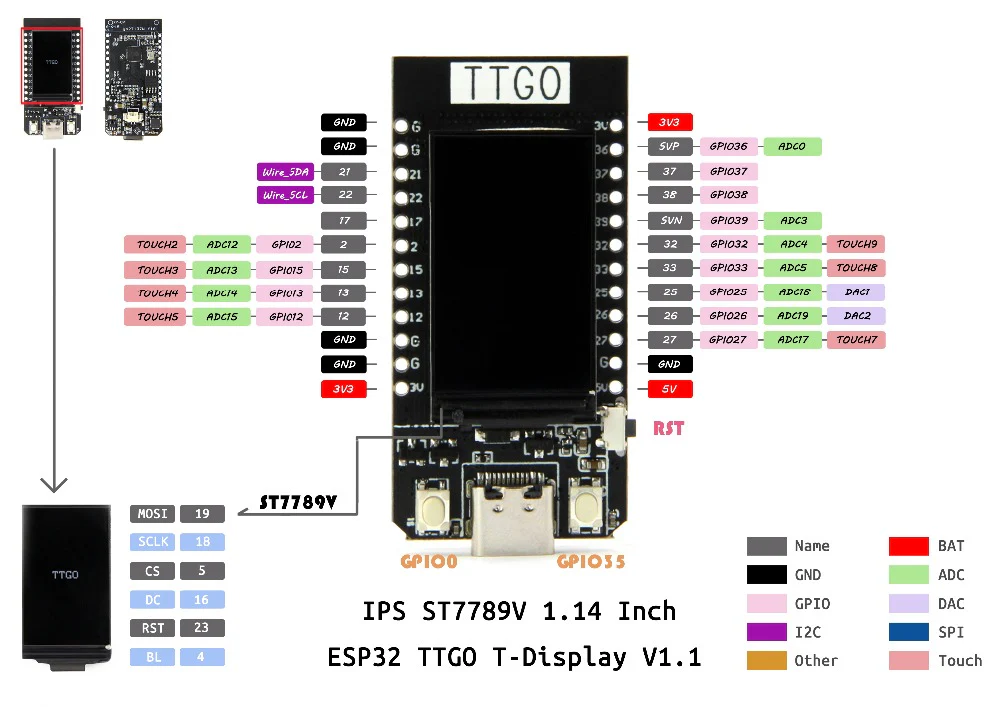
\includegraphics[width=1\textwidth]{development-testing/development/image/esp32ttgo_specification.png}
    \caption{TTGO T-Display ESP32 board specifications.}
    \label{fig:esp32ttgo_specification}
\end{figure}

The outputs of this phase directly constrain the mechanical design: every internal cavity, port cutout, and mounting feature in the housing must correspond to the physical layout established here. System analysis therefore acts as the foundational step that ensures dimensional accuracy and functional compatibility throughout the rest of the pipeline.
\subsection{Mechanical Design}

With the board's geometry fully characterised, the mechanical design phase produces the custom 3D-printed housing. The workflow within this phase proceeds through four successive steps.

\subsubsection{CAD Modelling}

The enclosure is modelled in Autodesk Fusion 360. The internal cavity is dimensioned to match the board footprint with controlled tolerances, while external features, including 

\begin{itemize}
    \item Side-wall apertures for the USB-C port and buttons
    \item Front-face opening for the display
\end{itemize}

are positioned to align with the results of the system analysis phase. Structural features such as snap-fit clips or interlocking tabs are added at this stage to facilitate tool-free assembly.

Throughout the CAD modelling process, DFA principles are applied to minimise part count and simplify the assembly procedure. The housing is consequently designed as a two-part clamshell (a front cover and a back shell) that snaps together without fasteners, eliminating screws and reducing the total component count.

\subsubsection{Slicing and Print-Parameter Configuration}

The finalised CAD model is exported and imported into Ultimaker Cura for slicing. Print parameters including layer height, infill density and pattern, wall line count, support structures, and print speed are configured to balance structural integrity, dimensional accuracy, and print time. The orientation of each part on the build plate is chosen to minimise the need for support material and to ensure that critical surfaces are printed at optimal quality.

\subsubsection{FDM Printing}

The sliced G-code files are transferred to a Creality Ender 3 V2 printer. As mentioned above, PLA filament is selected for its ease of printing, good dimensional stability, and sufficient mechanical strength for a non-load-bearing enclosure application. After printing, the parts undergo basic post-processing, removal of support material and light surface finishing, before proceeding to the integration phases.
\subsection{Electrical Integration}

Once the housing has been produced, the electrical integration phase establishes the physical connections required for a fully functional device. This phase begins with a detailed review of the board's I/O interfaces, power supply requirements, and pin assignments to identify any additional components or wiring needed. The necessary electrical connections between the ESP32 board and peripheral components are then designed and implemented, with attention given to cable routing within the enclosure so that connections do not obstruct assembly or the placement of the board inside the housing.
\subsection{Programming}

The project is built on the \textbf{Arduino framework} targeting the ESP32 microcontroller, compiled and flashed via the Arduino IDE 2.x with the official ESP32 board package. The primary display library is \textbf{TFT\_eSPI}, which provides hardware-accelerated, low-level access to the ST7789 controller of the built-in 1.14-inch TFT screen.

The firmware follows a simple \textbf{mode-switching} architecture centred on a single main loop. The concept of an \textit{active mode} is the central organising principle: a global state variable tracks which application or screen is currently displayed. Each iteration of the main loop routes control to the rendering and input-handling routine of that mode.

On startup, the device attempts to synchronise system time with an NTP server over Wi-Fi (allowing up to ten seconds). If synchronisation succeeds, the real-time clock is set accordingly; otherwise it falls back to the compile-time timestamp as a seed. After initialisation, the system enters its main loop, which continuously polls the two physical buttons (\texttt{GPIO0} and \texttt{GPIO35}), updates the active application, and redraws the display.

The home screen is divided into two regions. The upper area displays a live digital clock, showing hours, minutes, seconds, and the current date. Below it, a fixed navigation bar presents six application icons arranged in two rows of three. A single press on either button moves the selection highlight one slot in the corresponding direction (with wrap-around); a double press on either button launches the currently highlighted application.

The firmware ships with six self-contained applications accessible from the home screen:

\begin{itemize}
  \item \textbf{Stopwatch}: a centisecond-precision stopwatch with lap recording;
  \item \textbf{Calculator}: a four-function calculator with an on-screen 16-key grid;
  \item \textbf{Animation}: a looping sprite-sheet animation rendered from a compile-time frame header, convertible from a GIF;
  \item \textbf{Alien Attack}: a space-shooter arcade game in which the player dodges and shoots descending enemies;
  \item \textbf{Tetris}: a classic falling-block puzzle game;
  \item \textbf{Demo Image Viewer}: a viewer that cycles through full-screen RGB565 images stored in flash.
\end{itemize}

% \begin{figure}[H]
%     \centering
%     \begin{subfigure}[b]{0.1\textwidth}
%         \centering
%         
\includegraphics[width=\textwidth]{development-testing/development/image/program_stopwatch_icon.png}
%         \caption{Stopwatch}
%     \end{subfigure}
%     \hfill
%     \begin{subfigure}[b]{0.1\textwidth}
%         \centering
%         
\includegraphics[width=\textwidth]{development-testing/development/image/program_calculator_icon.png}
%         \caption{Calculator}
%     \end{subfigure}
%     \hfill
%     \begin{subfigure}[b]{0.1\textwidth}
%         \centering
%         
\includegraphics[width=\textwidth]{development-testing/development/image/program_animation_icon.png}
%         \caption{Animation}
%     \end{subfigure}
%     \hfill
%     \begin{subfigure}[b]{0.1\textwidth}
%         \centering
%         
\includegraphics[width=\textwidth]{development-testing/development/image/program_alienattack_icon.png}
%         \caption{Alien Attack}
%     \end{subfigure}
%     \hfill
%     \begin{subfigure}[b]{0.1\textwidth}
%         \centering
%         
\includegraphics[width=\textwidth]{development-testing/development/image/program_tetris_icon.png}
%         \caption{Tetris}
%     \end{subfigure}
%     \hfill
%     \begin{subfigure}[b]{0.1\textwidth}
%         \centering
%         
\includegraphics[width=\textwidth]{development-testing/development/image/program_image_icon.png}
%         \caption{Image Viewer}
%     \end{subfigure}
%     \label{fig:application_icons}
% \end{figure}

Each application is implemented as a self-contained module under its own subdirectory, exposing a rendering function and an input-handler function that the main loop calls during the corresponding mode. This modular layout keeps concerns separated and makes it straightforward to add or remove applications without modifying the core dispatch logic.